\section{Technical Documentation}

\subsection{Architecture} 
The image below gives an overview about the technologies that we have used in the development of the WeekMe application and where these are used within our overall system.   

	\begin{figure}[H] 
		\centering 
		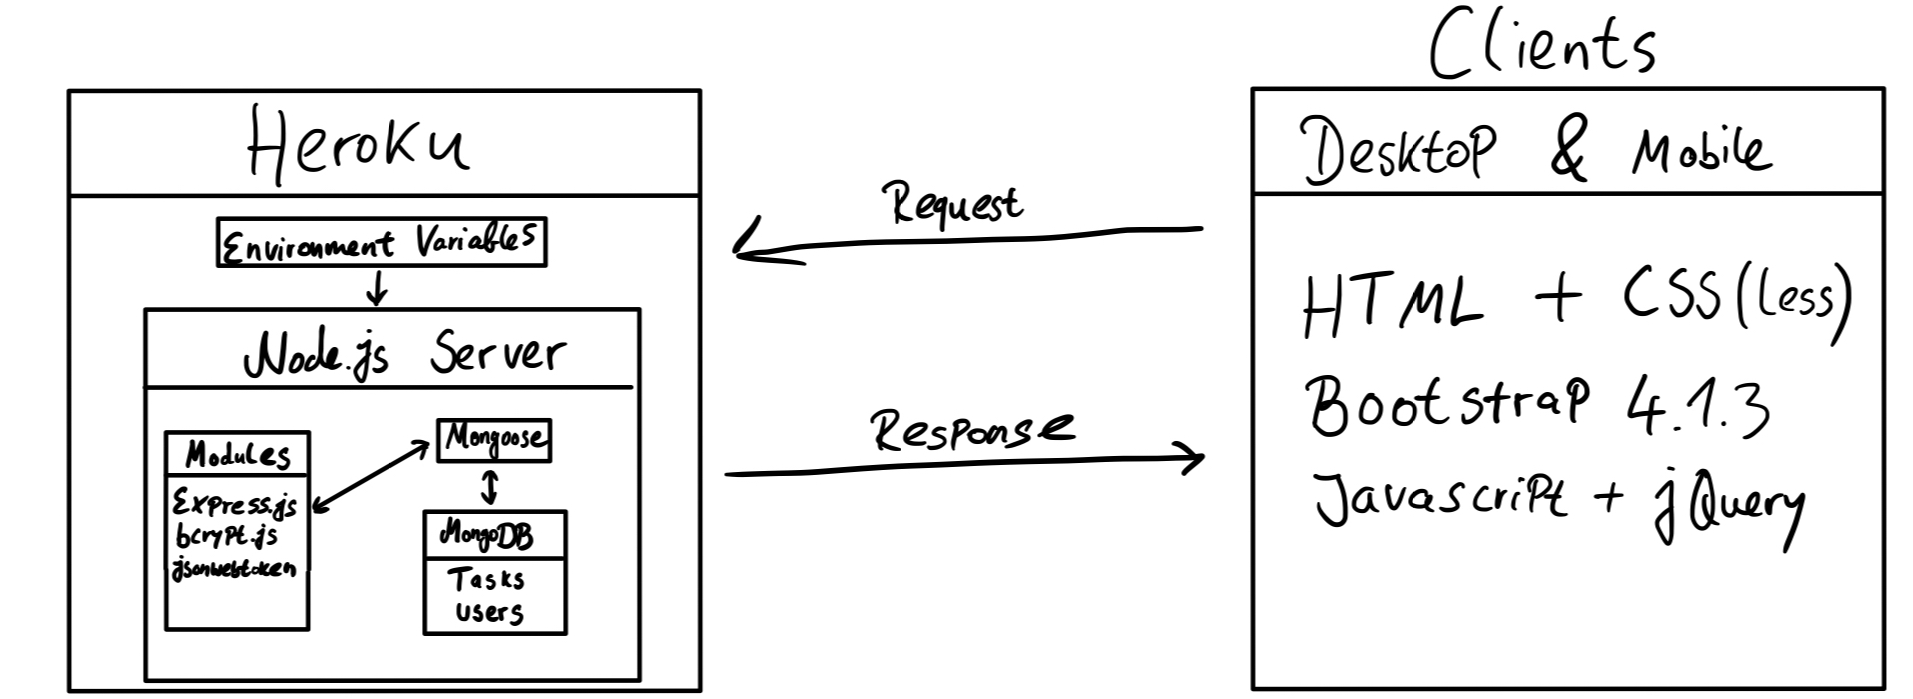
\includegraphics[height=6.2cm]{figures/architecture}    
		\caption{System Architecture}     
	\end{figure}  
 
\subsection{Backend} 

\subsubsection{Node.js}
The backbone of our backend is a node.js server. As node natively supports all the functionality we really need for our server we could use it by itself. Instead we chose to extend nodes functionality using express.js, as it generally makes development slightly faster.  

\myparagraph{Modules}   



\textbf{Express.js}  is one of the most popular modules available on npm. It is a server side web framework that extends the functionality of Node.js with many handy tools making development faster and easier. An express application consists of at least one file usually called app.js. This file registers any middleware and controllers the application is using. Furthermore the web-server is started here. A basic express web-server can be started in the following way:   

\begin{lstlisting}
const express = require("express");
var app = express();
app.listen(3000, () => {
  console.log("Server is up on port: ", 3000); 
});  
\end{lstlisting}    



\textbf{Routing} 
Routing is used to determine how our application responds to client requests at a particular endpoint.  
Typical client requests HTTP methods are GET, POST, PUT and DELETE. The initial setup of our routing is done using an instance of our express app. We can add routes and their handlers to our app in the following form:

\begin{lstlisting}
	app.METHOD(PATH, HANDLER); 
\end{lstlisting}

Where app is an instance of express, METHOD is an HTTP request method, PATH is a path on the server and HANDLER is the function executed when the route is matched. The simple examples below demonstrate a basic routing for each HTTP method type. In all of these cases our handler simply returns a string value to the client.   

\begin{lstlisting}
app.get('/', function (req, res) {
  res.send('Hello World!')
})

app.post('/', function (req, res) {
  res.send('Got a POST request')
})

app.put('/user', function (req, res) {
  res.send('Got a PUT request at /user')
})

app.delete('/user', function (req, res) {
  res.send('Got a DELETE request at /user')
})

\end{lstlisting}


\textbf{Serving static files}
In order to be able to serve static files our WeekMe application needs to be configured properly. The most common scenario in which we need to serve public files is when we want to include css, html or other resource files. We use an integrated express middleware function called "express.static" (as explained in the next section) to let our app know where to find our public directory containing the static files. Having done this clients are able to load files from the public directory.     

\begin{lstlisting}
	app.use(express.static('public'));  
\end{lstlisting}

\textbf{Express Middleware} lets us run certain code before or after certain events. Express middleware adds on to the express functionality. Middleware functions have access to the request and response object as well as the next middleware function in the execution cycle.  Common examples of things express middleware can do are:  

\begin{itemize}
	\item Execute Code
	\item Change to request or response objects
	\item Determine whether or not somebody is logged in and may access a page
	\item respond to a request 
\end{itemize}

The following middleware function is used inside the application to determine whether the user that is accessing the route is logged in.  

\begin{lstlisting}
var authenticate = (req, res, next) => {
  var token = req.header("x-auth");

  User.findByToken(token).then((user) => {
    if(!user){
      return Promise.reject();
    }
    req.user = user;
    req.token = token;
    next(); 
  }).catch((e) => {
    res.status(401).send();
  });
};
\end{lstlisting}  

After having defined our middleware function, we need to append it to one of our routes so that it will be executed when this route is being accessed.   

\begin{lstlisting}
//Tell route to use middleware authenticate
app.get("/users/me", authenticate, (req, res) => {
  //because we are using the middleware, we now have all the data we appended inside that middleware available here inside the req object
  res.send(req.user);
}); 
\end{lstlisting} 

\textbf{Bcrypt} is a module that can be used to hash passwords. Hashing passwords is considered a mandatory operation before storing them to a database in any secure and professional environment, as it prevents attackers that might get access to the dataset from reading and using any passwords that are stored. Hashing is a one way street and always returns the exact same hash for the same string. When hashing a password a salt is used to increase security even further. Salting password hashes is also considered mandatory. Otherwise we will always receive the same exact hash when using the same exact password. This would enable people to use a lookup table that maps thousands of common password phrases or english words to their hashes. Ultimately they would be able to get the password from the hash. Thats why an unknown salt is needed. Often a randomly generated value is used for the salting process. This ensures that will never receive the same value twice and prevents users from being able to trick us and change data by generating their own hashes. 

\begin{lstlisting}
// Hashing a password
bcrypt.hash('my password', 'my salt', (err, hash) => {
  // Store hash password in DB
});

//Checking a password
bcrypt.compare('my password', hash, (err, res) => {
  // res == true or res == false
});
\end{lstlisting}


\textbf{JsonWebToken} is yet another npm module that helps us to setup a secure environment for our application. Its main use case is generating unique tokens that can be used for user authentication. Once generated and assigned to a specific user, the tokens can be used to access private routes that could otherwise not be accessed. This way not anyone can make a HTTP request to our server and we make sure that only verified and authenticated requests are being made. In fact, most routes inside WeekMe will be private and only the login and signup routes will be public. In the code snipped below we use jsonwebtoken to create a token. When the token is decoded using jsonwebtokens verify method, we need to pass in the exact same salt that we used when creating the token, otherwise we will not be able to access the id and iat (=issuedAt) properties that are stored inside the data object.  

\begin{lstlisting}
const jwt = require("jsonwebtoken");

var data = {
  id: 10
};

var token = jwt.sign(data, "mysaltysalt");
console.log(token);
var decoded = jwt.verify (token, "mysaltysalt");
console.log("Decoded", decoded);  //Decoded --> {id: 10, iat: 1526910769}
\end{lstlisting}

\cleardoublepage 

We can visit \url{https://jwt.io } to get information about the hash we have created using the jsonwebtoken module. Each component of our token stores a different information. The red part is the header. The purple part is the payload storing the actual information (id, iat) and the blue part is the hash that lets us verify that the payload has never been changed. 

	\begin{figure}[H] 
		\centering 
		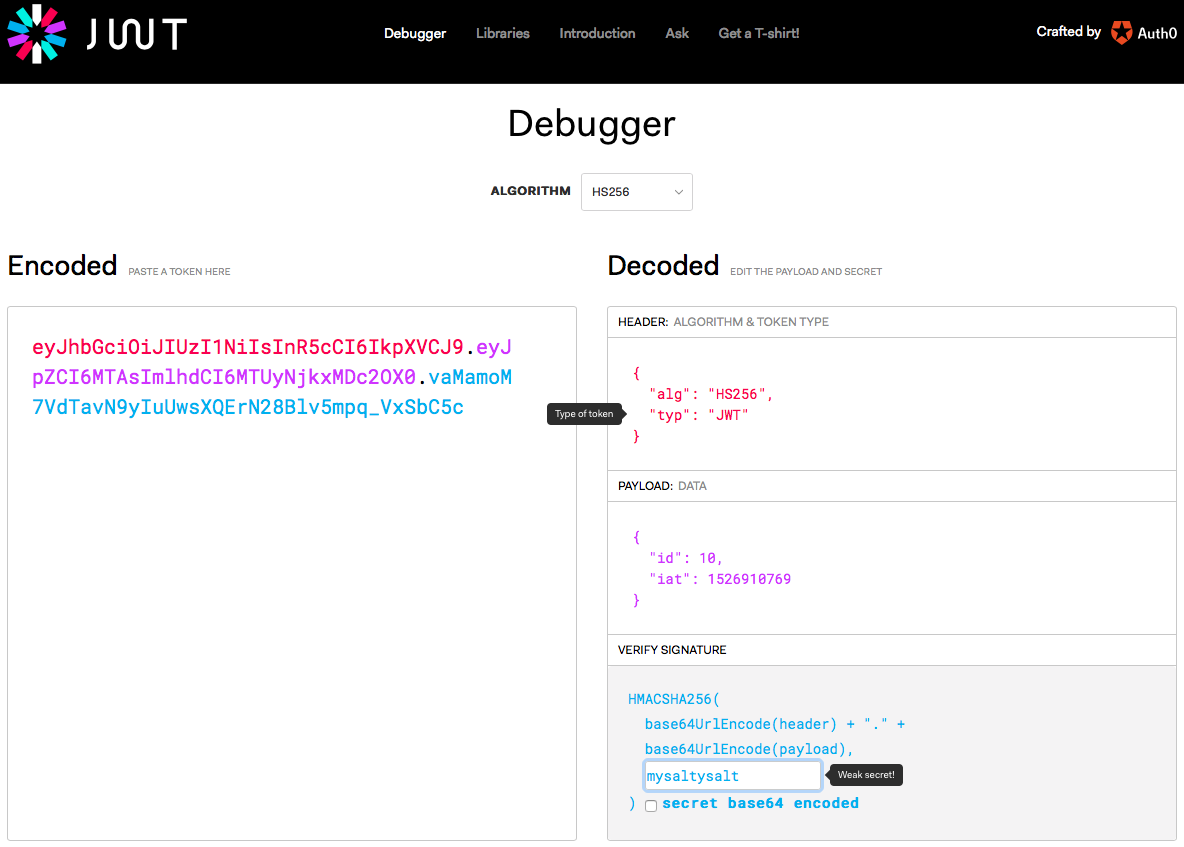
\includegraphics[height=10cm]{figures/jwt}    
		\caption[Jsonwebtoken info at: https://jwt.io]{Jsonwebtoken info at: https://jwt.io}     
		\label{fig: Jsonwebtoken info at: https://jwt.io}      
	\end{figure}    

 


When a user signs up, a unique token will be created and stored into the database. From now on this token is used for any authentication when accessing private routes instead of the email and password properties that have been provided by the user in the signup process. 

\begin{lstlisting}
UserSchema.methods.generateAuthToken = function () {
  var user = this; 
  var access = "auth";
  var token = jwt.sign({_id: user._id.toHexString(), access}, process.env.JWT_SECRET);

  user.tokens = user.tokens.concat([{access, token}]);
  return user.save().then(() => {
    return token;
  });
};

\end{lstlisting}


\cleardoublepage

\textbf{NodeMailer} is a popular NPM module that can be used to send emails from a node server. Within our application we have decided to use this library to be able to send out reset-password emails to our users in case they have forgotten their login password. In case a user does not click on the provided reset link inside the email the reset code in the database expires after an hour has passed. 

	\begin{figure}[H] 
		\centering 
		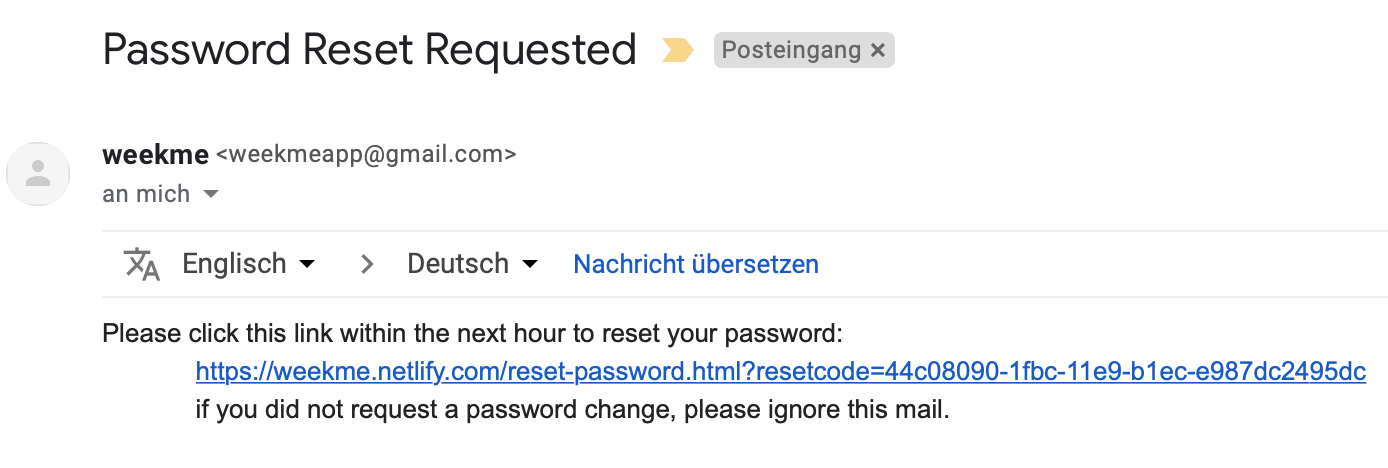
\includegraphics[height=4.5cm]{figures/passwordresetmail}    
		\caption{Reset Password Email}     
	\end{figure}  

	In order to send the emails we created a new gmail account and applied the required configuration steps that enable our account to be accessed by our WeekMe API server. Finally we created the EmailSender module where we provided the login credentials. In order to exclude the gmail account password from the repository we stored it inside a Heroku environment variable that we can access from within our code (see line 5 below). Next to the initial configuration the EmailSender module also contains a basic implementation to send out said emails to our users.   
	
	\begin{lstlisting} 
	var transporter = nodemailer.createTransport({
    	service: 'gmail',
    	auth: {
     	 user: 'weekmeapp@gmail.com',
     	 pass: process.env.GMAILPASSWORD
    	}
	})
	\end{lstlisting} 

\subsubsection{Heroku}
Heroku is a handy and powerful online platform that enables us to easily deploy and test our applications in the cloud. Once we have setup our account on Heroku.com a series of terminal commands is required in order to get our application up and running on Heroku. The first step is to login to our Heroku account inside of the terminal. 

\begin{verbatim}
	$ heroku login
\end{verbatim}

Once we are logged in we have to add our public ssh key to Heroku.

\begin{verbatim}
	$ heroku keys:add
\end{verbatim}

If we would like to delete a key from Heroku we use the following command while providing the corresponding email address. 
\begin{verbatim}
	$ heroku keys:remove example@mail.com 
\end{verbatim}

We can check for any keys linked to the Heroku account in the following way.
\begin{verbatim}
	$ heroku keys 
\end{verbatim}

In order to create a new application in Heroku and link it to our Git repository we use the create command. 
\begin{verbatim}
	$ heroku create
\end{verbatim}

When we want to deploy our application to Heroku we simply need to push it to the heroku branch that has been created in the last step. 
\begin{verbatim}
	$ git push heroku
\end{verbatim}

Using the heroku open command a browser window with our application will be launched.
\begin{verbatim}
	$ heroku open
\end{verbatim}

In order to make sure that heroku is actually launching the correct file we need to edit the package.json file and go to the scripts section. In there we edit the value of the start property to launch the server. 

\begin{lstlisting}
  ...
  "scripts": {
    "test": "echo \"Error: no test specified\" && exit 1",
    "start": "node server.js"  // Heroku will execute this line on startup  
  } 
  ...
\end{lstlisting} 


\subsubsection{Making the App Secure}
In order to have a truly secure application we need make sure that no sensitive information like API keys or passwords are stored inside the code. For that matter we create a config.js file that will be added to the .gitignore file to exclude it from being pushed to our repository. Sensitive data should not be pushed to the repository because anybody that has access to the repository will be able to see it.   
 
\begin{lstlisting}
//config.json 
{
  "development": {
    "PORT": 3000, 
    "MONGODB_URI": "mongodb://localhost:27017/WeekMe",
    "JWT_SECRET": "asdahjsdajsdbhjg1hjdhj1"
  }
} 
\end{lstlisting}


One way to remove sensitive information from our code is to use environment variables. 
In the code snipped below we set the environment variable depending on whether we are in our development (localhost) or production (Heroku) environment. 

\begin{lstlisting}
config.js
var env = process.env.NODE_ENV || "development";  
console.log("env ***** ", env);
if(env === "development" || env === "test"){
  var config = require("./config.json"); //When using require on a json file it will automatically be converted to a javascript object.
  var envConfig = config[env]; //get env property of config
  Object.keys(envConfig).forEach((key) => {
    process.env[key] = envConfig[key];
  });
}
\end{lstlisting}
 
Once we have assigned all keys to the process.env variable we may access them from anywhere inside our code. 

\begin{lstlisting}
	var token = jwt.sign({_id: user._id.toHexString(), access}, process.env.JWT_SECRET);
\end{lstlisting}

Last but not least we need to make sure that Heroku is also provided with an environment variable storing the JWT\_SECRET value so that the application may function properly in production.  

	\begin{figure}[H] 
		\centering 
		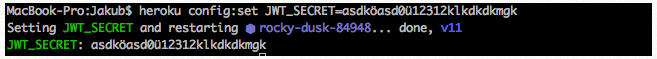
\includegraphics[height=1.4cm]{figures/herokuenvironmentvar}    
		\caption[Setting an environment variable in Heroku]{Setting an environment variable in Heroku}     
		\label{fig: Setting an environment variable in Heroku}     
	\end{figure}  


\subsubsection{MongoDB \& Mongoose} 
All data that is created by WeekMe is stored inside a MongoDB database instance. As MongoDB works very well together with node and due to the fact that our entire business logic is coded in JavaScript we decided to use a JSON style document based database. This allows for easy transformation from the JavaScript objects to JSON and vice versa reducing development time and the amount of code.  
  

\subsection{Frontend}
Apart from HTML, CSS and JavaScript WeekMe makes use of the following technologies. 
\subsubsection{Technologies}
\paragraph{Bootstrap}\mbox{}\\
Bootstrap is an open source toolkit used to build responsive, mobile-first projects on the web. 
It is the world’s most popular front-end component library. WeekMe makes use of its grid-layout, modals, navigation bar and buttons.
\cite{bootstrap}

\paragraph{less}\mbox{}\\
Leaner Styles Sheets (less) is a backwards-compatible language extension for CSS. It adds features like variables, mixins and functions.
\cite{less}
The stylesheets used for designing WeekMe are generated from less code. 

\paragraph{jQuery}\mbox{}\\
jQuery is a fast and feature-rich JavaScript library. It makes things like HTML document manipulation and traversal, animations and event handling simpler. It is very popular and works with a multitude of browsers.
\cite{jquery}
In WeekMe it is mainly used to help querying and manipulating the DOM (Document Object Model) and adding event handlers. 

\subsubsection{Calling our API}

\subsubsection{Picker Popup} 
To create a new task or to edit an existing task we decided to create an overlaying popup window with several creating steps. \\
We wanted the creation process to be as easy and fast as possible to reduce the needed afford and enable a quick usage. \\
So we split the process in three steps: \\
Step one: The popup window opens with a customised headline, a textarea for the task-description, a coloured button for the color picker, a button for the day picker if you want to choose another day as pre-selected and a done button to create the save the task immediately. \\
In step one it’s required to enter a task-description. The options to choose a color for the task or a day in which the task will be saved are optional. So if the user clicks the done button immediately after he typed a description the task will be saved with the pre-selected color and the pre-selected day. \\
On the other hand the user can decide to change the color and press the button which is coloured in the selected color of the task in the left bottom corner of the popup window. This will trigger step two in which the user can choose the color for the task. The popup window for step one will disappear and the color picker popup will appear. After the user clicks on one of the six color buttons or the back button, step two will disappear and the step one will be shown again with an updated color picker button and the task description you entered before. \\
To enter step three you have to click on the “another day” button to open the day picker popup. Now you can choose another day or the stack out of a dropdown menu to save the task to. Then you can finish the creation process with a click on done or you can enter step one again if you click back. In this case the day picker will be reset. \\
To realise such a popup window we used the “modal” component from bootstrap. The advantage of using this modal is that it is responsive, so it works and looks good on any device or browser. \\  
At first the html-code of all three steps of the picker-popup is created and will be inserted to the DOM. This is realised in the functions createModal() and insertModal(). The picker to select the day the task will be added to is created and inserted right after the modal creation at the functions createPicker() and insertPicker(). How the days are arranged at the dropdown menu depends on the current day. The pre-selected day is the day you clicked on to starting the task creating process. The functions createPicker() and insertPicker() will be executed at other points of the program to reset the picker options and the selected day. \\
To open the task creation popup you have to call the showPicker() function of the ui\_picker.js document. Depending on how you make the call the picker will occur in different shapes. The  popup style depends on which button you clicked at the surface. If you want to edit a task, create a task at a specific day or create a task in general. The difference between the shown popups are the headline, color, existing task-description and which buttons are shown. I implemented some shortcut buttons who were planned to be used in the case the user wants to create a task not related to a certain day. We didn’t implemented such a button for day-independent-task-creation without a preselection yet. This option was not necessary at this point, but we look forward to implement this as well. Cause these Shortcut buttons are designed to assign the created task with one click to the current day or to the stack, which we expect will be the most used options, so the user don’t have to go over to the third popup-window, where they can choose another day. This will shorten the time of task creation and improve the user experience. To prove our expectation we look forward to use these already implemented but hidden shortcut buttons to run some A/B-testing.





